\documentclass[11pt,a4paper]{article}
\usepackage[utf8]{inputenc}
\usepackage[margin=0.85in]{geometry}
\usepackage{amsmath,amssymb,amsthm}
\usepackage{xcolor}
\usepackage{tcolorbox}
\usepackage{tikz}
\usetikzlibrary{shapes,arrows,positioning,calc,decorations.pathreplacing}
\usepackage{booktabs}
\usepackage{array}
\usepackage{fancyhdr}
\usepackage{hyperref}
\usepackage{microtype}

% Color Palette Definitions
\definecolor{primarynavy}{RGB}{26, 54, 93}       % #1A365D - Deep Navy
\definecolor{secondaryteal}{RGB}{13, 148, 136}   % #0D9488 - Teal Accent
\definecolor{darkslate}{RGB}{45, 55, 72}        % #2D3748 - Body Text
\definecolor{lightbg}{RGB}{247, 250, 252}        % #F7FAFC - Soft Background
\definecolor{accentblue}{RGB}{49, 130, 206}      % #3182CE - Bright Blue
\definecolor{warmgold}{RGB}{214, 158, 46}        % #D69E2E - Gold Highlight

\hypersetup{
    colorlinks=true,
    linkcolor=primarynavy,
    citecolor=secondaryteal,
    urlcolor=accentblue,
    pdftitle={Comprehensive Lecture Notes: Numerical Analysis},
    pdfauthor={Class Notes}
}

% Page Setup
\pagestyle{fancy}
\fancyhf{}
\fancyhead[L]{\small \textbf{\color{primarynavy}Numerical Analysis: Rigorous Derivations \& Error Analysis}}
\fancyhead[R]{\small \textbf{\color{secondaryteal}MATMJ54}}
\fancyfoot[L]{\small \textcolor{primarynavy}{\href{https://www.sciqb.com}{\textbf{www.sciqb.com}}}}
\fancyfoot[C]{\thepage}
\fancyfoot[R]{\small \textcolor{secondaryteal}{\href{https://www.sciqb.com}{\textbf{SCIQB Platform}}}}
\renewcommand{\headrulewidth}{0.6pt}
\renewcommand{\footrulewidth}{0.4pt}

% Custom TColorBox Environments
\newtcolorbox{defbox}[1]{
    colback=lightbg,
    colframe=primarynavy,
    fonttitle=\bfseries\color{white},
    title={#1},
    boxrule=1pt,
    top=3mm, bottom=3mm, left=4mm, right=4mm
}

\newtcolorbox{formulabox}[1]{
    colback=secondaryteal!8!white,
    colframe=secondaryteal,
    fonttitle=\bfseries\color{white},
    title={#1},
    boxrule=1pt,
    top=3mm, bottom=3mm, left=4mm, right=4mm
}

\newtcolorbox{exbox}[1]{
    colback=white,
    colframe=accentblue,
    fonttitle=\bfseries\color{white},
    title={#1},
    boxrule=1pt,
    top=3mm, bottom=3mm, left=4mm, right=4mm
}

\setlength{\parindent}{0pt}
\setlength{\parskip}{6pt}

\begin{document}

% Title Banner
\begin{center}
    \tcbset{colframe=primarynavy,colback=primarynavy!5!white,arc=0mm}
    \begin{tcolorbox}[sharp corners, boxrule=1.5pt]
        \begin{center}
            {\Large \bfseries \color{primarynavy} COMPLETE MATHEMATICAL LECTURE NOTES ON NUMERICAL ANALYSIS}\\[4pt]
            {\large \bfseries \color{secondaryteal} Exhaustive Step-by-Step Algebraic Derivations, Taylor Expansions, Error Proofs \& Visual Graphs}\\[6pt]
            {\small \textbf{Course Code:} MATMJ54 \quad|\quad \textbf{Platform:} \href{https://www.sciqb.com}{\color{accentblue}\textbf{www.sciqb.com}}}
        \end{center}
    \end{tcolorbox}
\end{center}

\vspace{0.3cm}

\tableofcontents
\newpage

\section{Module 1: Errors and Their Computations}

Numerical methods approximate continuous mathematical operations using discrete computational algorithms. A fundamental part of numerical analysis is evaluating, bounding, and minimizing errors.

\subsection{Classification of Numerical Errors}

\begin{enumerate}
    \item \textbf{Inherent / Initial Errors:} Errors present in the raw input data prior to calculation due to physical measurement limits or empirical approximations.
    \item \textbf{Truncation Errors:} Errors introduced when an infinite mathematical operation is approximated by a finite sequence of operations (e.g., truncating an infinite Taylor series).
    \item \textbf{Round-off Errors:} Errors caused by representing real numbers with finite machine precision (floating-point representation) in computing systems.
\end{enumerate}

\subsection{Mathematical Definitions of Error}

\begin{defbox}{Definitions: Error Metrics}
Let $X$ denote the exact true value of a quantity and $X^*$ denote its approximate value.
\begin{itemize}
    \item \textbf{Absolute Error ($E_A$):}
    \begin{equation}
        E_A = |X - X^*|
    \end{equation}
    
    \item \textbf{Relative Error ($E_R$):}
    \begin{equation}
        E_R = \frac{|X - X^*|}{|X|} = \frac{E_A}{|X|}, \quad (X \neq 0)
    \end{equation}
    
    \item \textbf{Percentage Error ($E_P$):}
    \begin{equation}
        E_P = E_R \times 100\% = \frac{|X - X^*|}{|X|} \times 100\%
    \end{equation}
\end{itemize}
\end{defbox}

\subsection{Significant Digits and Error Bounds}

\begin{formulabox}{Theorem: Significant Digits Error Bound}
An approximate number $X^*$ is said to be correct to $n$ decimal places (or significant digits) if the absolute error is bounded by:
\begin{equation}
    E_A = |X - X^*| \le \frac{1}{2} \times 10^{-n}
\end{equation}
If $X^*$ is rounded to $n$ decimal places, the maximum truncation/rounding error is $\frac{1}{2} \cdot 10^{-n}$.
\end{formulabox}

\newpage

\section{Module 2: Bisection and Regula-Falsi Methods}

\subsection{Intermediate Value Theorem (IVT)}

\begin{defbox}{Intermediate Value Theorem}
If $f(x)$ is continuous on a closed interval $[a, b]$ and $f(a) \cdot f(b) < 0$ (meaning $f(a)$ and $f(b)$ have opposite signs), then there exists at least one root $\alpha \in (a, b)$ such that $f(\alpha) = 0$.
\end{defbox}

\subsection{Bisection Method}

The Bisection Method repeatedly halves the bracket interval $[a, b]$.

\begin{center}
\begin{tikzpicture}[scale=1.1]
    \draw[->,thick] (-0.5,0) -- (5.5,0) node[right] {$x$};
    \draw[->,thick] (0,-1.5) -- (0,2.5) node[above] {$y$};
    \draw[smooth,domain=0.5:4.8,thick,primarynavy] plot (\x,{0.3*(\x-1)*(\x-3)*(\x-4.5) + 0.2*(\x-2.5)});
    \draw[dashed,darkslate] (1,0) node[below] {$a_0$} -- (1,-1.15);
    \draw[dashed,darkslate] (4.5,0) node[below] {$b_0$} -- (4.5,1.9);
    \draw[dashed,secondaryteal] (2.75,0) node[above] {$c_0 = \frac{a_0+b_0}{2}$} -- (2.75,-0.55);
    \filldraw[secondaryteal] (2.75,0) circle (2pt);
    \filldraw[accentblue] (3.08,0) circle (2pt) node[below=4pt] {$\alpha$};
\end{tikzpicture}
\end{center}

\begin{formulabox}{Bisection Iteration Formula and Error Bound Proof}
Midpoint formula: $c_k = \frac{a_k + b_k}{2}$.

\textbf{Complete Step-by-Step Proof of Error Bound $|c_n - \alpha| \le \frac{b-a}{2^n}$:}
\begin{enumerate}
    \item \textbf{Initial Step ($n=0$):} The initial interval is $[a_0, b_0]$ with length $b_0 - a_0 = b - a$.
    \item \textbf{Interval Halving after $n$ Steps:} At each successive iteration, the interval is halved:
    $$\text{Length of } [a_n, b_n] = b_n - a_n = \frac{b - a}{2^n}$$
    \item \textbf{Root Proximity to Midpoint:} Since $f(a_n) f(b_n) < 0$, the exact root $\alpha$ lies inside $[a_n, b_n]$. The midpoint $c_n = \frac{a_n + b_n}{2}$ is at the center of $[a_n, b_n]$. Thus, the distance between $c_n$ and any point in $[a_n, b_n]$ cannot exceed half the interval length:
    \begin{equation}
        |c_n - \alpha| \le \frac{b_n - a_n}{2} = \frac{b - a}{2^{n+1}} \le \frac{b - a}{2^n} \quad \qed
    \end{equation}
\end{enumerate}
\textbf{Rate of Convergence:} The Bisection method converges \textbf{linearly} with order $p = 1$ and asymptotic error constant $C = 1/2$.
\end{formulabox}

\newpage

\subsection{Regula-Falsi (False Position) Method}

\begin{center}
\begin{tikzpicture}[scale=1.1]
    \draw[->,thick] (-0.5,0) -- (5.5,0) node[right] {$x$};
    \draw[->,thick] (0,-2) -- (0,2.5) node[above] {$y$};
    \draw[smooth,domain=0.5:5,thick,primarynavy] plot (\x,{0.25*(\x-3)^3 + 0.4*(\x-3)});
    \filldraw[primarynavy] (1,-1.6) circle (2pt) node[left] {$(a, f(a))$};
    \filldraw[primarynavy] (4.5,1.8) circle (2pt) node[right] {$(b, f(b))$};
    \draw[thick,secondaryteal] (1,-1.6) -- (4.5,1.8);
    \filldraw[warmgold] (2.64,0) circle (2.5pt) node[below=2pt] {$c$};
    \filldraw[accentblue] (3,0) circle (2pt) node[above right] {$\alpha$};
\end{tikzpicture}
\end{center}

\begin{defbox}{Regula-Falsi Formula}
The secant line connecting $(a, f(a))$ and $(b, f(b))$ has equation:
\begin{equation}
    y - f(a) = \frac{f(b) - f(a)}{b - a} (x - a)
\end{equation}
Setting $y = 0$ gives the root approximation $c$:
\begin{equation}
    c = \frac{a f(b) - b f(a)}{f(b) - f(a)} = a - \frac{b - a}{f(b) - f(a)} f(a)
\end{equation}
\end{defbox}

\subsubsection{Exhaustive Step-by-Step Proof of Regula-Falsi Linear Convergence}

\textbf{Setting:} Let $\alpha$ be the exact root ($f(\alpha) = 0$). In the Regula-Falsi method, one of the bracket endpoints remains fixed (say $x_0 = a = \alpha + e_0$, where $e_0$ is the constant error of the fixed endpoint), while the other endpoint $x_k = \alpha + e_k$ moves towards $\alpha$.

\begin{exbox}{Step 1: Set up the Error Recurrence Equation}
Substitute $x_k = \alpha + e_k$, $x_0 = \alpha + e_0$, and $x_{k+1} = \alpha + e_{k+1}$ into the iteration formula:
\begin{align}
    x_{k+1} &= x_k - \frac{x_k - x_0}{f(x_k) - f(x_0)} f(x_k) \notag \\
    \alpha + e_{k+1} &= (\alpha + e_k) - \frac{(\alpha + e_k) - (\alpha + e_0)}{f(\alpha + e_k) - f(\alpha + e_0)} f(\alpha + e_k) \notag \\
    e_{k+1} &= e_k - (e_k - e_0) \frac{f(\alpha + e_k)}{f(\alpha + e_k) - f(\alpha + e_0)}
\end{align}
\end{exbox}

\begin{exbox}{Step 2: Taylor Series Expansions about the Exact Root $\alpha$}
Since $f(\alpha) = 0$, expanding $f(\alpha + e_k)$ and $f(\alpha + e_0)$ in Taylor series gives:
\begin{align}
    f(\alpha + e_k) &= e_k f'(\alpha) + \frac{e_k^2}{2!} f''(\alpha) + \frac{e_k^3}{3!} f'''(\alpha) + \dots \notag \\
    &= e_k f'(\alpha) \left[ 1 + \frac{1}{2} e_k \frac{f''(\alpha)}{f'(\alpha)} + \frac{1}{6} e_k^2 \frac{f'''(\alpha)}{f'(\alpha)} + \dots \right]
\end{align}
Similarly for the fixed endpoint:
\begin{equation}
    f(\alpha + e_0) = e_0 f'(\alpha) + \frac{e_0^2}{2!} f''(\alpha) + \frac{e_0^3}{3!} f'''(\alpha) + \dots
\end{equation}
Subtracting $f(\alpha + e_0)$ from $f(\alpha + e_k)$ for the denominator:
\begin{align}
    f(\alpha + e_k) - f(\alpha + e_0) &= (e_k - e_0) f'(\alpha) + \frac{e_k^2 - e_0^2}{2!} f''(\alpha) + \frac{e_k^3 - e_0^3}{3!} f'''(\alpha) + \dots \notag \\
    &= (e_k - e_0) f'(\alpha) \left[ 1 + \frac{1}{2}(e_k + e_0)\frac{f''(\alpha)}{f'(\alpha)} + \frac{1}{6}(e_k^2 + e_k e_0 + e_0^2)\frac{f'''(\alpha)}{f'(\alpha)} + \dots \right]
\end{align}
\end{exbox}

\newpage

\begin{exbox}{Step 3: Canceling Common Factors and Applying Binomial Expansion}
Substitute equations (9) and (11) into the error formula:
\begin{align}
    e_{k+1} &= e_k - (e_k - e_0) \frac{e_k f'(\alpha) \left[ 1 + \frac{1}{2} e_k \frac{f''(\alpha)}{f'(\alpha)} + \frac{1}{6} e_k^2 \frac{f'''(\alpha)}{f'(\alpha)} + \dots \right]}{(e_k - e_0) f'(\alpha) \left[ 1 + \frac{1}{2}(e_k + e_0)\frac{f''(\alpha)}{f'(\alpha)} + \frac{1}{6}(e_k^2 + e_k e_0 + e_0^2)\frac{f'''(\alpha)}{f'(\alpha)} + \dots \right]} \notag \\
    &= e_k - e_k \left[ 1 + \frac{1}{2} e_k \frac{f''(\alpha)}{f'(\alpha)} + \frac{1}{6} e_k^2 \frac{f'''(\alpha)}{f'(\alpha)} + \dots \right] \notag \\
    &\quad \times \left[ 1 + \frac{1}{2}(e_k + e_0)\frac{f''(\alpha)}{f'(\alpha)} + \frac{1}{6}(e_k^2 + e_k e_0 + e_0^2)\frac{f'''(\alpha)}{f'(\alpha)} + \dots \right]^{-1}
\end{align}
Using the Binomial expansion identity $(1 + u)^{-1} = 1 - u + u^2 - \dots$:
\begin{align}
    &\left[ 1 + \frac{1}{2}(e_k + e_0)\frac{f''(\alpha)}{f'(\alpha)} + \frac{1}{6}(e_k^2 + e_k e_0 + e_0^2)\frac{f'''(\alpha)}{f'(\alpha)} + \dots \right]^{-1} \notag \\
    &= 1 - \left\{ \frac{1}{2}(e_k + e_0)\frac{f''(\alpha)}{f'(\alpha)} + \frac{1}{6}(e_k^2 + e_k e_0 + e_0^2)\frac{f'''(\alpha)}{f'(\alpha)} \right\} + \left\{ \frac{1}{2}(e_k + e_0)\frac{f''(\alpha)}{f'(\alpha)} \right\}^2 - \dots
\end{align}
\end{exbox}

\begin{exbox}{Step 4: Term-by-Term Cross Multiplication and Simplification}
Multiplying the two bracketed series:
\begin{align}
    &= 1 + \frac{1}{2} e_k \frac{f''(\alpha)}{f'(\alpha)} + \frac{1}{6} e_k^2 \frac{f'''(\alpha)}{f'(\alpha)} - \frac{1}{2}(e_k + e_0)\frac{f''(\alpha)}{f'(\alpha)} - \frac{1}{6}(e_k^2 + e_k e_0 + e_0^2)\frac{f'''(\alpha)}{f'(\alpha)} \notag \\
    &\quad - \frac{1}{4} e_k(e_k + e_0)\left(\frac{f''(\alpha)}{f'(\alpha)}\right)^2 + \frac{1}{4}(e_k^2 + 2e_k e_0 + e_0^2)\left(\frac{f''(\alpha)}{f'(\alpha)}\right)^2 + \dots \notag \\
    &= 1 + \frac{1}{2}\{ e_k - (e_k + e_0) \}\frac{f''(\alpha)}{f'(\alpha)} + (e_k e_0 + e_0^2)\left[ \frac{1}{4}\left(\frac{f''(\alpha)}{f'(\alpha)}\right)^2 - \frac{1}{6}\frac{f'''(\alpha)}{f'(\alpha)} \right] + \dots \notag \\
    &= 1 - \frac{1}{2} e_0 \frac{f''(\alpha)}{f'(\alpha)} + (e_k e_0 + e_0^2)\left[ \frac{1}{4}\left(\frac{f''(\alpha)}{f'(\alpha)}\right)^2 - \frac{1}{6}\frac{f'''(\alpha)}{f'(\alpha)} \right] + \dots
\end{align}
Substitute this expression back into the equation for $e_{k+1}$:
\begin{align}
    e_{k+1} &= e_k - e_k \left[ 1 - \frac{1}{2} e_0 \frac{f''(\alpha)}{f'(\alpha)} + (e_k e_0 + e_0^2)\left\{ \frac{1}{4}\left(\frac{f''(\alpha)}{f'(\alpha)}\right)^2 - \frac{1}{6}\frac{f'''(\alpha)}{f'(\alpha)} \right\} + \dots \right] \notag \\
    &= e_k - e_k + e_k e_0 \frac{f''(\alpha)}{2 f'(\alpha)} + (e_k^2 e_0 + e_k e_0^2)\left[ \frac{1}{6}\frac{f'''(\alpha)}{f'(\alpha)} - \frac{1}{4}\left(\frac{f''(\alpha)}{f'(\alpha)}\right)^2 \right] + \dots \notag \\
    \mathbf{e_{k+1}} &= \mathbf{e_k e_0 \frac{f''(\alpha)}{2 f'(\alpha)} + O(e_k^2 e_0 + e_k e_0^2)}
\end{align}
\end{exbox}

\begin{exbox}{Step 5: Order of Convergence Conclusion}
Since the initial endpoint $x_0 = a$ is fixed throughout the iterations, $e_0$ is a non-zero constant. Defining $A = \frac{e_0 f''(\alpha)}{2 f'(\alpha)}$:
\begin{equation}
    e_{k+1} = A e_k
\end{equation}
Comparing with the general error relation $|e_{k+1}| = C |e_k|^p$ gives $p = 1$.
$$\mathbf{\text{Rate of Convergence of Regula-Falsi Method is } p = 1 \text{ (Linear Convergence)}} \quad \qed$$
\end{exbox}

\newpage

\section{Module 3: Secant Method and Rate of Convergence}

\subsection{Derivation and Iteration Formula}

\begin{center}
\begin{tikzpicture}[scale=1.1]
    \draw[->,thick] (-0.5,0) -- (5.5,0) node[right] {$x$};
    \draw[->,thick] (0,-2) -- (0,2.5) node[above] {$y$};
    \draw[smooth,domain=0.5:5,thick,primarynavy] plot (\x,{0.3*(\x-2.8)^3 + 0.5*(\x-2.8)});
    \filldraw[primarynavy] (1,-1.9) circle (2pt) node[below left] {$(x_0, f(x_0))$};
    \filldraw[primarynavy] (4.5,2.1) circle (2pt) node[above right] {$(x_1, f(x_1))$};
    \draw[thick,secondaryteal] (0.8,-2.14) -- (4.8,2.44);
    \filldraw[warmgold] (2.66,0) circle (2.5pt) node[above left] {$x_2$};
    \filldraw[accentblue] (2.8,0) circle (2pt) node[below right] {$\alpha$};
\end{tikzpicture}
\end{center}

\begin{defbox}{Secant Method Iteration}
Unlike Regula-Falsi, the Secant Method does not require bracketing $f(x_{k-1})f(x_k) < 0$. It draws a secant line through the two most recent iterates $(x_{k-1}, f(x_{k-1}))$ and $(x_k, f(x_k))$:
\begin{equation}
    x_{k+1} = x_k - \frac{x_k - x_{k-1}}{f(x_k) - f(x_{k-1})} f(x_k), \quad k = 1, 2, 3, \dots
\end{equation}
\end{defbox}

\subsection{\texorpdfstring{Exhaustive Proof: Rate of Convergence of Secant Method ($p \approx 1.6180$)}{Exhaustive Proof: Rate of Convergence of Secant Method (p = 1.6180)}}

\begin{exbox}{Step 1 to 3: Error Recurrence and Asymptotic Form}
\textbf{Step 1: Write Error Recurrence Relation}
Let $x_{k-1} = \alpha + e_{k-1}, x_k = \alpha + e_k, x_{k+1} = \alpha + e_{k+1}$:
\begin{equation}
    e_{k+1} = e_k - (e_k - e_{k-1}) \frac{f(\alpha + e_k)}{f(\alpha + e_k) - f(\alpha + e_{k-1})}
\end{equation}

\textbf{Step 2: Taylor Expansion \& Asymptotic Error Relation}
Following the exact algebraic simplification as derived in Module 2, but with the moving iterate $e_{k-1}$ in place of the fixed $e_0$:
\begin{equation}
    e_{k+1} = e_k e_{k-1} \frac{f''(\alpha)}{2 f'(\alpha)} + O(e_k^2 e_{k-1} + e_k e_{k-1}^2)
\end{equation}
Defining asymptotic error constant $A = \frac{f''(\alpha)}{2 f'(\alpha)}$:
\begin{equation}
    e_{k+1} \approx A e_k e_{k-1} \quad \text{--- (Equation 1)}
\end{equation}

\textbf{Step 3: Postulate the Order of Convergence Relation}
Assume an error relation of the form:
\begin{equation}
    e_{k+1} = c e_k^p \quad \text{--- (Equation 2)}
\end{equation}
where $c$ is a constant and $p$ is the order of convergence.
Expressing $e_k$ and $e_{k-1}$ from Equation (2):
\begin{align}
    e_k &= c^{-1/p} e_{k+1}^{1/p} \notag \\
    e_{k-1} &= c^{-1/p} e_k^{1/p} \quad \text{--- (Equation 3)}
\end{align}
\end{exbox}

\begin{exbox}{Step 4 to 5: Characteristic Exponent Equation and Root Calculation}
\textbf{Step 4: Substitute Equations (2) and (3) into Equation (1)}
\begin{align}
    c e_k^p &= A e_k \left( c^{-1/p} e_k^{1/p} \right) \notag \\
    c^{1 + 1/p} e_k^p &= A e_k^{1 + 1/p}
\end{align}

\textbf{Step 5: Equate Exponents of $e_k$ and Solve the Characteristic Equation}
Equating the exponents of $e_k$ on both sides:
\begin{align}
    p &= 1 + \frac{1}{p} \notag \\
    p^2 - p - 1 &= 0 \notag \\
    p &= \frac{-(-1) \pm \sqrt{(-1)^2 - 4(1)(-1)}}{2(1)} = \frac{1 \pm \sqrt{1 + 4}}{2} = \frac{1 \pm \sqrt{5}}{2}
\end{align}
Evaluating the roots:
\begin{itemize}
    \item $p_1 = \frac{1 - \sqrt{5}}{2} = \frac{1 - 2.236068}{2} \approx -0.61803$ (Discard negative root)
    \item $p_2 = \frac{1 + \sqrt{5}}{2} = \frac{1 + 2.236068}{2} \approx \mathbf{1.61803}$
\end{itemize}
$$\mathbf{\text{Rate of Convergence of Secant Method is } p = \frac{1+\sqrt{5}}{2} \approx 1.6180 \text{ (Superlinear / Golden Ratio)}} \quad \qed$$
\end{exbox}

\newpage

\subsection{Solved Example: Regula-Falsi vs. Secant Method}

\begin{exbox}{Comparative Worked Example: $f(x) = x^3 + x^2 - 1 = 0$ on $[0, 1]$}
Observe $f(0) = 0^3 + 0^2 - 1 = -1 < 0$ and $f(1) = 1^3 + 1^2 - 1 = 1 > 0$. The root lies in $[0, 1]$.

\textbf{1. Regula-Falsi Method ($a=0, b=1$):}
\begin{itemize}
    \item $k=1$: $c = \frac{0(1) - 1(-1)}{1 - (-1)} = \frac{1}{2} = 0.5$. $f(0.5) = 0.5^3 + 0.5^2 - 1 = -0.625 < 0 \implies [0.5, 1]$
    \item $k=2$: $c = \frac{0.5(1) - 1(-0.625)}{1 - (-0.625)} = \frac{1.125}{1.625} \approx 0.692307$. $f(0.692307) = -0.188916 \implies [0.692307, 1]$
    \item $k=3$: $c = \frac{0.692307(1) - 1(-0.188916)}{1 - (-0.188916)} = \frac{0.881223}{1.188916} \approx 0.741198$. $f(0.741198) = -0.043430 \implies [0.741198, 1]$
    \item $k=4$: $c = \frac{0.741198(1) - 1(-0.043430)}{1 + 0.043430} \approx 0.751969$. $f(0.751969) = -0.009336 \implies [0.751969, 1]$
    \item $k=5$: $c = \frac{0.751969(1) - 1(-0.009336)}{1 + 0.009336} \approx \mathbf{0.754263}$.
\end{itemize}

\textbf{2. Secant Method ($x_0 = 0, x_1 = 1$):}
\begin{itemize}
    \item $x_0 = 0, f(x_0) = -1$
    \item $x_1 = 1, f(x_1) = 1$
    \item $x_2 = 1 - \frac{1 - 0}{1 - (-1)}(1) = 1 - 0.5 = 0.5, \quad f(0.5) = -0.625$
    \item $x_3 = 0.5 - \frac{0.5 - 1}{-0.625 - 1}(-0.625) = 0.5 + \frac{-0.5}{-1.625}(-0.625) = 0.692307, \quad f(x_3) = -0.188916$
    \item $x_4 = 0.692307 - \frac{0.692307 - 0.5}{-0.188916 - (-0.625)}(-0.188916) = 0.692307 + \frac{0.192307(0.188916)}{0.436084} \approx 0.775607, \quad f(x_4) = 0.066472$
    \item $x_5 = 0.775607 - \frac{0.775607 - 0.692307}{0.066472 - (-0.188916)}(0.066472) \approx \mathbf{0.753951}$.
\end{itemize}
\end{exbox}

\newpage

\section{Module 4: Newton-Raphson Method and Applications}

\subsection{Derivation and Tangent Formula}

\begin{center}
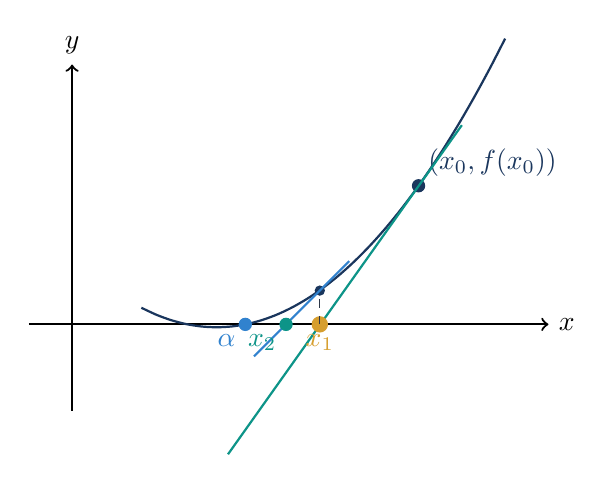
\begin{tikzpicture}[scale=1.1]
    \draw[->,thick] (-0.5,0) -- (5.5,0) node[right] {$x$};
    \draw[->,thick] (0,-1) -- (0,3) node[above] {$y$};
    \draw[smooth,domain=0.8:5,thick,primarynavy] plot (\x,{0.3*(\x-2)^2 + 0.2*(\x-2)});
    \filldraw[primarynavy] (4,1.6) circle (2pt) node[above right] {$(x_0, f(x_0))$};
    \draw[thick,secondaryteal] (1.8,-1.5) -- (4.5,2.3);
    \filldraw[warmgold] (2.86,0) circle (2.5pt) node[below] {$x_1$};
    \draw[dashed,darkslate] (2.86,0) -- (2.86,0.39);
    \filldraw[primarynavy] (2.86,0.39) circle (1.5pt);
    \draw[thick,accentblue] (2.1,-0.37) -- (3.2,0.73);
    \filldraw[secondaryteal] (2.47,0) circle (2pt) node[below left] {$x_2$};
    \filldraw[accentblue] (2,0) circle (2pt) node[below left] {$\alpha$};
\end{tikzpicture}
\end{center}

\begin{formulabox}{Newton-Raphson Formula}
Let $x_0$ be an initial guess for the root of $f(x) = 0$. The tangent line to $y = f(x)$ at $(x_0, f(x_0))$ is:
\begin{equation}
    y - f(x_0) = f'(x_0)(x - x_0)
\end{equation}
Setting $y = 0$ gives the first approximation $x_1$:
\begin{equation}
    0 - f(x_0) = f'(x_0)(x_1 - x_0) \implies x_1 = x_0 - \frac{f(x_0)}{f'(x_0)}
\end{equation}
Iterating $k$ times gives the general Newton-Raphson formula:
\begin{equation}
    x_{k+1} = x_k - \frac{f(x_k)}{f'(x_k)}, \quad f'(x_k) \neq 0
\end{equation}
\end{formulabox}

\subsection{\texorpdfstring{Exhaustive Proof: Quadratic Convergence ($p = 2$)}{Exhaustive Proof: Quadratic Convergence (p = 2)}}

\begin{exbox}{Step 1: Set up Error Expression from Iteration Formula}
Let $\alpha$ be the exact root such that $f(\alpha) = 0$. Let $x_k = \alpha + e_k$ and $x_{k+1} = \alpha + e_{k+1}$, where $e_k$ and $e_{k+1}$ are the errors at steps $k$ and $k+1$:
\begin{align}
    \alpha + e_{k+1} &= \alpha + e_k - \left[ \frac{f(\alpha + e_k)}{f'(\alpha + e_k)} \right] \notag \\
    e_{k+1} &= e_k - \frac{f(\alpha + e_k)}{f'(\alpha + e_k)}
\end{align}
\end{exbox}

\begin{exbox}{Step 2: Taylor Expansions of $f(\alpha + e_k)$ and $f'(\alpha + e_k)$ up to 3rd Derivative}
Expanding $f(\alpha + e_k)$ and $f'(\alpha + e_k)$ about $\alpha$ in Taylor series:
\begin{align}
    f(\alpha + e_k) &= f(\alpha) + e_k f'(\alpha) + \frac{e_k^2}{2!} f''(\alpha) + \frac{e_k^3}{3!} f'''(\alpha) + \dots \notag \\
    f'(\alpha + e_k) &= f'(\alpha) + e_k f''(\alpha) + \frac{e_k^2}{2!} f'''(\alpha) + \dots
\end{align}
Since $\alpha$ is a root of $f(x) = 0$, substitute $f(\alpha) = 0$:
\begin{equation}
    e_{k+1} = e_k - \frac{\left[ e_k f'(\alpha) + \frac{e_k^2}{2!} f''(\alpha) + \frac{e_k^3}{3!} f'''(\alpha) + \dots \right]}{\left[ f'(\alpha) + e_k f''(\alpha) + \frac{1}{2} e_k^2 f'''(\alpha) + \dots \right]}
\end{equation}
\end{exbox}

\newpage

\begin{exbox}{Step 3: Factoring $f'(\alpha)$ out of Numerator and Denominator}
Factor out $e_k f'(\alpha)$ from the numerator and $f'(\alpha)$ from the denominator:
\begin{align}
    e_{k+1} &= e_k - \frac{e_k f'(\alpha) \left[ 1 + \frac{e_k}{2!} \frac{f''(\alpha)}{f'(\alpha)} + \frac{e_k^2}{3!} \frac{f'''(\alpha)}{f'(\alpha)} + \dots \right]}{f'(\alpha) \left[ 1 + \left\{ e_k \frac{f''(\alpha)}{f'(\alpha)} + \frac{1}{2} e_k^2 \frac{f'''(\alpha)}{f'(\alpha)} + \dots \right\} \right]} \notag \\
    &= e_k - e_k \left[ 1 + \frac{1}{2} e_k \frac{f''(\alpha)}{f'(\alpha)} + \frac{1}{6} e_k^2 \frac{f'''(\alpha)}{f'(\alpha)} + \dots \right] \times \left[ 1 + \left\{ e_k \frac{f''(\alpha)}{f'(\alpha)} + \frac{1}{2} e_k^2 \frac{f'''(\alpha)}{f'(\alpha)} \right\} \right]^{-1}
\end{align}
\end{exbox}

\begin{exbox}{Step 4: Applying Binomial Series Expansion $(1 + u)^{-1} = 1 - u + u^2 - \dots$}
Expanding the inverted denominator using the binomial expansion:
\begin{align}
    &\left[ 1 + \left\{ e_k \frac{f''(\alpha)}{f'(\alpha)} + \frac{1}{2} e_k^2 \frac{f'''(\alpha)}{f'(\alpha)} \right\} \right]^{-1} \notag \\
    &= 1 - \left\{ e_k \frac{f''(\alpha)}{f'(\alpha)} + \frac{1}{2} e_k^2 \frac{f'''(\alpha)}{f'(\alpha)} + \dots \right\} + \left\{ e_k \frac{f''(\alpha)}{f'(\alpha)} + \frac{1}{2} e_k^2 \frac{f'''(\alpha)}{f'(\alpha)} + \dots \right\}^2 - \dots \notag \\
    &= 1 - e_k \frac{f''(\alpha)}{f'(\alpha)} - \frac{1}{2} e_k^2 \frac{f'''(\alpha)}{f'(\alpha)} + e_k^2 \left(\frac{f''(\alpha)}{f'(\alpha)}\right)^2 - \dots
\end{align}
\end{exbox}

\begin{exbox}{Step 5: Full Term-by-Term Cross Multiplication}
Multiplying the two series expansion brackets together:
\begin{align}
    &= \left[ 1 + \frac{1}{2} e_k \frac{f''(\alpha)}{f'(\alpha)} + \frac{1}{6} e_k^2 \frac{f'''(\alpha)}{f'(\alpha)} + \dots \right] \times \left[ 1 - e_k \frac{f''(\alpha)}{f'(\alpha)} - \frac{1}{2} e_k^2 \frac{f'''(\alpha)}{f'(\alpha)} + e_k^2 \left(\frac{f''(\alpha)}{f'(\alpha)}\right)^2 - \dots \right] \notag \\
    &= 1 + e_k \left\{ \frac{1}{2} - 1 \right\} \frac{f''(\alpha)}{f'(\alpha)} + e_k^2 \left\{ \frac{1}{6}\frac{f'''(\alpha)}{f'(\alpha)} - \frac{1}{2}\left(\frac{f''(\alpha)}{f'(\alpha)}\right)^2 - \frac{1}{2}\frac{f'''(\alpha)}{f'(\alpha)} + \left(\frac{f''(\alpha)}{f'(\alpha)}\right)^2 \right\} + \dots \notag \\
    &= 1 - \frac{1}{2} e_k \frac{f''(\alpha)}{f'(\alpha)} + e_k^2 \left\{ \left(\frac{1}{6} - \frac{1}{2}\right)\frac{f'''(\alpha)}{f'(\alpha)} + \left(1 - \frac{1}{2}\right)\left(\frac{f''(\alpha)}{f'(\alpha)}\right)^2 \right\} + \dots \notag \\
    &= 1 - \frac{1}{2} e_k \frac{f''(\alpha)}{f'(\alpha)} + e_k^2 \left\{ -\frac{1}{3}\frac{f'''(\alpha)}{f'(\alpha)} + \frac{1}{2}\left(\frac{f''(\alpha)}{f'(\alpha)}\right)^2 \right\} + \dots
\end{align}
\end{exbox}

\begin{exbox}{Step 6: Substituting into $e_{k+1}$ and Final Order of Convergence}
Substituting the product back into the $e_{k+1}$ equation:
\begin{align}
    e_{k+1} &= e_k - e_k \left[ 1 - \frac{1}{2} e_k \frac{f''(\alpha)}{f'(\alpha)} + e_k^2 \left\{ -\frac{1}{3}\frac{f'''(\alpha)}{f'(\alpha)} + \frac{1}{2}\left(\frac{f''(\alpha)}{f'(\alpha)}\right)^2 \right\} + \dots \right] \notag \\
    &= e_k - e_k + \frac{e_k^2}{2} \frac{f''(\alpha)}{f'(\alpha)} + e_k^3 \left\{ \frac{1}{3}\frac{f'''(\alpha)}{f'(\alpha)} - \frac{1}{2}\left(\frac{f''(\alpha)}{f'(\alpha)}\right)^2 \right\} + \dots \notag \\
    &= \frac{f''(\alpha)}{2 f'(\alpha)} e_k^2 + e_k^3 \left\{ \frac{1}{3}\frac{f'''(\alpha)}{f'(\alpha)} - \frac{1}{2}\left(\frac{f''(\alpha)}{f'(\alpha)}\right)^2 \right\} + \dots \notag \\
    \mathbf{e_{k+1}} &= \mathbf{\frac{f''(\alpha)}{2 f'(\alpha)} e_k^2 + O(e_k^3)}
\end{align}
Defining asymptotic error constant $C = \left| \frac{f''(\alpha)}{2 f'(\alpha)} \right|$:
\begin{equation}
    |e_{k+1}| \le C |e_k|^2 \implies \mathbf{p = 2 \quad \text{(Quadratic Order of Convergence)}} \quad \qed
\end{equation}
\end{exbox}

\newpage

\subsection{Solved Newton-Raphson Polynomial Examples}

\begin{exbox}{Example 1: $f(x) = x^3 + x^2 - 1 = 0$}
Given $f(x) = x^3 + x^2 - 1 \implies f'(x) = 3x^2 + 2x$.
Iteration formula:
\begin{equation}
    x_{k+1} = x_k - \frac{x_k^3 + x_k^2 - 1}{3x_k^2 + 2x_k} = \frac{3x_k^3 + 2x_k^2 - x_k^3 - x_k^2 + 1}{3x_k^2 + 2x_k} = \mathbf{\frac{2x_k^3 + x_k^2 + 1}{3x_k^2 + 2x_k}}
\end{equation}
Let initial approximation $x_0 = 1$:
\begin{itemize}
    \item $k=0$: $x_1 = \frac{2(1)^3 + 1^2 + 1}{3(1)^2 + 2(1)} = \frac{4}{5} = \mathbf{0.8}$
    \item $k=1$: $x_2 = \frac{2(0.8)^3 + 0.8^2 + 1}{3(0.8)^2 + 2(0.8)} = \frac{2(0.512) + 0.64 + 1}{3(0.64) + 1.6} = \frac{1.024 + 0.64 + 1}{1.92 + 1.6} = \frac{2.664}{3.52} \approx \mathbf{0.756818}$
    \item $k=2$: $x_3 = \frac{2(0.756818)^3 + (0.756818)^2 + 1}{3(0.756818)^2 + 2(0.756818)} \approx \mathbf{0.754878}$
\end{itemize}

\textbf{Practice Problems:}
\begin{enumerate}
    \item $x^3 - 2x - 5 = 0$
    \item $x^3 + 4x^2 - 3x + 1 = 0$
    \item $x^3 - 5x + 3 = 0$
\end{enumerate}
\end{exbox}

\subsection{Special Newton-Raphson Algorithms}

\begin{formulabox}{1. Cube Root Algorithm ($\sqrt[3]{N}$)}
Let $x = \sqrt[3]{N} \implies x^3 = N \implies f(x) = x^3 - N = 0, \quad f'(x) = 3x^2$.
Newton-Raphson formula:
\begin{equation}
    x_{k+1} = x_k - \frac{x_k^3 - N}{3x_k^2} = \frac{3x_k^3 - x_k^3 + N}{3x_k^2} = \mathbf{\frac{2x_k^3 + N}{3x_k^2}}
\end{equation}

\textbf{Numerical Example: Find $\sqrt[3]{37}$ using Newton-Raphson}
\begin{itemize}
    \item Let $f(x) = x^3 - 37 = 0$.
    \item Test integers: $f(3) = 3^3 - 37 = 27 - 37 = -10 < 0$ and $f(4) = 4^3 - 37 = 64 - 37 = 27 > 0$.
    \item Root lies in $[3, 4]$. Choose initial guess $x_0 = 3$.
    \item Iteration formula: $x_{k+1} = \frac{2x_k^3 + 37}{3x_k^2}$.
    \item $k=0$: $x_1 = \frac{2(3)^3 + 37}{3(3)^2} = \frac{2(27) + 37}{3(9)} = \frac{54 + 37}{27} = \frac{91}{27} \approx \mathbf{3.370370}$
    \item $k=1$: $x_2 = \frac{2(3.370370)^3 + 37}{3(3.370370)^2} = \frac{2(38.2854) + 37}{3(11.3594)} = \frac{113.5708}{34.0782} \approx \mathbf{3.332611}$
\end{itemize}
\end{formulabox}

\newpage

\begin{formulabox}{\texorpdfstring{2. Division-Free Reciprocal Algorithm ($1/N$) and Full Convergence Range Proof}{2. Division-Free Reciprocal Algorithm (1/N) and Full Convergence Range Proof}}
To find the reciprocal $x = 1/N$ without performing hardware division:
Let $f(x) = \frac{1}{x} - N = 0 \implies f'(x) = -\frac{1}{x^2}$.
\begin{equation}
    x_{k+1} = x_k - \frac{\frac{1}{x_k} - N}{-\frac{1}{x_k^2}} = x_k + x_k^2 \left(\frac{1}{x_k} - N\right) = x_k + x_k - N x_k^2 = \mathbf{2x_k - N x_k^2}
\end{equation}

\begin{center}
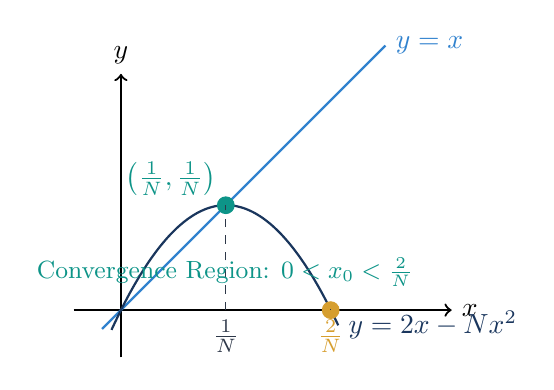
\begin{tikzpicture}[scale=1.2]
    \draw[->,thick] (-0.5,0) -- (3.5,0) node[right] {$x$};
    \draw[->,thick] (0,-0.5) -- (0,2.5) node[above] {$y$};
    \draw[thick,accentblue,domain=-0.2:2.8] plot (\x,\x) node[right] {$y = x$};
    \draw[smooth,domain=-0.1:2.3,thick,primarynavy] plot (\x,{2*\x - 0.9*\x*\x}) node[right] {$y = 2x - Nx^2$};
    \filldraw[secondaryteal] (1.11,1.11) circle (2.5pt) node[above left] {$\left(\frac{1}{N}, \frac{1}{N}\right)$};
    \filldraw[warmgold] (2.22,0) circle (2.5pt) node[below] {$\frac{2}{N}$};
    \draw[dashed,darkslate] (1.11,0) node[below] {$\frac{1}{N}$} -- (1.11,1.11);
    \draw[dashed,darkslate] (2.22,0) -- (2.22,0.01);
    \node[secondaryteal,font=\small] at (1.1, 0.4) {Convergence Region: $0 < x_0 < \frac{2}{N}$};
\end{tikzpicture}
\end{center}

\textbf{Geometric Analysis of Iteration Function:}
The iteration curve is the downward parabola $y = 2x - N x^2$:
$$y = -N\left(x^2 - \frac{2x}{N}\right) = -N\left[\left(x - \frac{1}{N}\right)^2 - \frac{1}{N^2}\right] \implies y - \frac{1}{N} = -N\left(x - \frac{1}{N}\right)^2$$
The vertex is located at $\left(\frac{1}{N}, \frac{1}{N}\right)$ and the parabola crosses the $x$-axis at $x = 0$ and $x = \frac{2}{N}$.

\textbf{Full Algebraic Proof that Convergence Requires $0 < x_0 < \frac{2}{N}$:}
\begin{enumerate}
    \item Define error at iteration $k+1$: $e_{k+1} = \frac{1}{N} - x_{k+1}$.
    \begin{align}
        e_{k+1} &= \frac{1}{N} - (2x_k - N x_k^2) = \frac{1}{N} - 2x_k + N x_k^2 \notag \\
        &= N \left( \frac{1}{N^2} - \frac{2x_k}{N} + x_k^2 \right) = N \left( \frac{1}{N} - x_k \right)^2 = \mathbf{N e_k^2}
    \end{align}
    \item Multiplying both sides by $N$:
    \begin{equation}
        N e_{k+1} = (N e_k)^2 = (N e_{k-1})^4 = \dots = (N e_0)^{2^{k+1}}
    \end{equation}
    \item For the error sequence to converge to zero ($e_k \to 0$ as $k \to \infty$), the base must satisfy:
    \begin{align}
        |N e_0| < 1 &\iff \left| N \left(\frac{1}{N} - x_0\right) \right| < 1 \notag \\
        &\iff |1 - N x_0| < 1 \notag \\
        &\iff -1 < 1 - N x_0 < 1 \notag \\
        &\iff -2 < -N x_0 < 0 \notag \\
        &\iff \mathbf{0 < x_0 < \frac{2}{N}} \quad \qed
    \end{align}
\end{enumerate}
\end{formulabox}

\newpage

\section{Module 5: Fixed-Point Iteration Method}

\subsection{Formulation and Cobweb Diagram}

\begin{center}
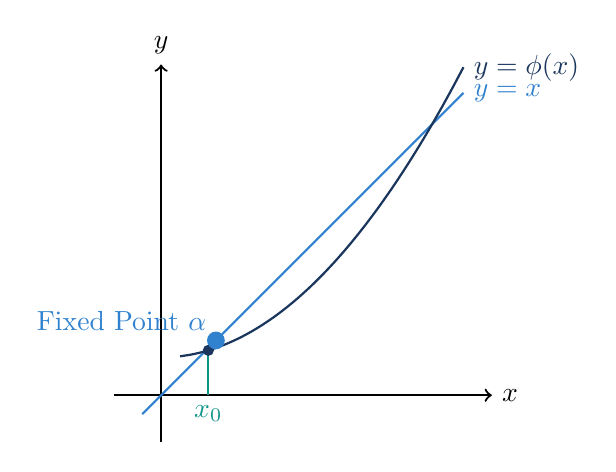
\begin{tikzpicture}[scale=1.2]
    \draw[->,thick] (-0.5,0) -- (3.5,0) node[right] {$x$};
    \draw[->,thick] (0,-0.5) -- (0,3.5) node[above] {$y$};
    \draw[thick,accentblue,domain=-0.2:3.2] plot (\x,\x) node[right] {$y = x$};
    \draw[smooth,domain=0.2:3.2,thick,primarynavy] plot (\x,{0.3*\x*\x + 0.4}) node[right] {$y = \phi(x)$};
    \draw[thick,secondaryteal] (0.5,0) node[below] {$x_0$} -- (0.5,0.475) -- (0.475,0.475) -- (0.475,0.467) -- (0.467,0.467);
    \filldraw[primarynavy] (0.5,0.475) circle (1.5pt);
    \filldraw[accentblue] (0.58,0.58) circle (2.5pt) node[above left] {Fixed Point $\alpha$};
\end{tikzpicture}
\end{center}

\begin{defbox}{Fixed-Point Iteration Scheme}
Given an equation $f(x) = 0$, rewrite it in the equivalent fixed-point form:
\begin{equation}
    x = \phi(x)
\end{equation}
Starting from an initial guess $x_0$, generate successive approximations:
\begin{align}
    \text{First approximation:} \quad x_1 &= \phi(x_0) \notag \\
    \text{Second approximation:} \quad x_2 &= \phi(x_1) \notag \\
    \text{Third approximation:} \quad x_3 &= \phi(x_2) \notag \\
    &\vdots \notag \\
    \text{$n$-th approximation:} \quad x_n &= \phi(x_{n-1}), \quad n = 1, 2, 3, \dots
\end{align}
\end{defbox}

\subsection{Exhaustive Step-by-Step Proof: Fixed-Point Convergence Theorem}

\begin{defbox}{Theorem Statement: Fixed-Point Iteration Convergence}
\textbf{Theorem:} If
\begin{enumerate}
    \item[(i)] $\alpha$ be a root of $f(x) = 0$, which is equivalent to $x = \phi(x)$.
    \item[(ii)] $I$ be any interval containing the root point $x = \alpha$.
    \item[(iii)] $|\phi'(x)| < 1$ for all $x \in I$.
\end{enumerate}
Then the sequence of iterative approximations $x_0, x_1, x_2, \dots, x_n, \dots$ will converge to the root $\alpha$, provided the initial approximation $x_0$ is chosen in $I$.
\end{defbox}

\begin{exbox}{Step 1 to 3: Setting Up Successive Differences}
\textbf{Step 1: Root Condition}
Since $\alpha$ is the exact root, it satisfies the fixed-point equation $x = \phi(x)$:
\begin{equation}
    \alpha = \phi(\alpha) \quad \text{--- (1)}
\end{equation}

\textbf{Step 2: Iteration Condition}
If $x_{n-1}$ and $x_n$ be two successive approximations to the root $\alpha$, then:
\begin{equation}
    x_n = \phi(x_{n-1}) \quad \text{--- (2)}
\end{equation}

\textbf{Step 3: Subtract Equation (1) from Equation (2)}
Subtracting (1) from (2) gives:
\begin{equation}
    x_n - \alpha = \phi(x_{n-1}) - \phi(\alpha) \quad \text{--- (3)}
\end{equation}
\end{exbox}

\newpage

\begin{exbox}{Step 4 to 6: Mean Value Theorem Application and Contraction Inequality}
\textbf{Step 4: Application of Lagrange's Mean Value Theorem}
By Lagrange's Mean Value Theorem, there exists a point $\xi$ strictly between $x_{n-1}$ and $\alpha$ such that:
\begin{equation}
    \frac{\phi(x_{n-1}) - \phi(\alpha)}{x_{n-1} - \alpha} = \phi'(\xi) \implies \phi(x_{n-1}) - \phi(\alpha) = (x_{n-1} - \alpha)\phi'(\xi)
\end{equation}

\textbf{Step 5: Substitute into Equation (3)}
\begin{equation}
    x_n - \alpha = (x_{n-1} - \alpha)\phi'(\xi)
\end{equation}
Taking the absolute value on both sides:
\begin{equation}
    |x_n - \alpha| = |x_{n-1} - \alpha| \cdot |\phi'(\xi)| \quad \text{--- (4)}
\end{equation}

\textbf{Step 6: Bound by Contraction Factor $k$}
Given that $|\phi'(x)| \le k < 1$ for all $x \in I$, and since $\xi \in I$, we have $|\phi'(\xi)| \le k$:
\begin{equation}
    |x_n - \alpha| \le k |x_{n-1} - \alpha| \quad \text{--- (5)}
\end{equation}
\end{exbox}

\begin{exbox}{Step 7 to 9: Backward Induction, Limit as $n \to \infty$ and Convergence Rate}
\textbf{Step 7: Recursive Substitution (Backward Induction)}
In Equation (5), replace $n$ by $n-1$:
\begin{equation}
    |x_{n-1} - \alpha| \le k |x_{n-2} - \alpha|
\end{equation}
Substituting this back into (5):
\begin{equation}
    |x_n - \alpha| \le k \cdot \left[ k |x_{n-2} - \alpha| \right] = k^2 |x_{n-2} - \alpha|
\end{equation}
Similarly, continuing this process recursively for $n-2, n-3, \dots, 0$:
\begin{equation}
    |x_n - \alpha| \le k^n |x_0 - \alpha|
\end{equation}

\textbf{Step 8: Taking Limit as $n \to \infty$}
Since $0 \le k < 1$, as $n \to \infty$, $k^n \to 0$:
\begin{equation}
    \lim_{n \to \infty} |x_n - \alpha| \le |x_0 - \alpha| \lim_{n \to \infty} k^n = 0
\end{equation}
\begin{equation}
    \Rightarrow \lim_{n \to \infty} x_n = \alpha
\end{equation}
Therefore, the sequence of approximations converges towards the exact root $\alpha$.

\textbf{Step 9: Rate of Convergence}
Let $e_n$ and $e_{n-1}$ be the errors in the $n$-th and $(n-1)$-th iterations:
$$e_n = x_n - \alpha, \quad e_{n-1} = x_{n-1} - \alpha$$
From Equation (5):
\begin{equation}
    |e_n| \le k |e_{n-1}|
\end{equation}
Comparing with standard error recurrence $|e_n| = C |e_{n-1}|^p$:
$$\mathbf{\text{Rate of Convergence of Fixed-Point Iteration is } p = 1 \text{ (Linear Convergence)}} \quad \qed$$
\end{exbox}

\newpage

\subsection{Solved Fixed-Point Iteration Examples}

\begin{exbox}{Example 1: Solve $x^3 - 3x + 1 = 0$ on $[0, 1]$}
\textbf{Step 1: Check Interval Signs}
$f(0) = 0^3 - 3(0) + 1 = 1 > 0$ and $f(1) = 1^3 - 3(1) + 1 = -1 < 0$. Root lies in $[0, 1]$.

\textbf{Step 2: Formulate $\phi(x)$ and Check Convergence Condition}
Rewrite $x^3 - 3x + 1 = 0 \implies 3x = x^3 + 1 \implies x = \phi(x) = \frac{1}{3}(x^3 + 1)$.
Compute derivative:
$$\phi'(x) = \frac{1}{3}(3x^2) = x^2$$
On $[0, 1)$, $|\phi'(x)| = x^2 < 1$. Thus, the iteration will converge!

\textbf{Step 3: Perform Iterations starting from $x_0 = 0$}
\begin{itemize}
    \item $n=1$: $x_1 = \phi(x_0) = \frac{1}{3}(0^3 + 1) = \frac{1}{3} \approx \mathbf{0.333333}$
    \item $n=2$: $x_2 = \phi(x_1) = \frac{1}{3}((0.333333)^3 + 1) = \frac{1}{3}(0.037037 + 1) = \frac{1.037037}{3} \approx \mathbf{0.345679}$
    \item $n=3$: $x_3 = \phi(x_2) = \frac{1}{3}((0.345679)^3 + 1) = \frac{1}{3}(0.041306 + 1) = \frac{1.041306}{3} \approx \mathbf{0.347098}$
\end{itemize}
\end{exbox}

\begin{exbox}{Example 2: Determine Parameter $K$ for $x^3 - 15 = 0$ on $[2, 3]$}
\textbf{Problem Statement:} Solve $x^3 - 15 = 0$ on $[2, 3]$ using the iteration form $x = \phi(x) = x + \frac{1}{K}(15 - x^3)$. Find an integer $K$ ensuring convergence.

\textbf{Step 1: Check Interval Signs}
$f(2) = 2^3 - 15 = 8 - 15 = -7 < 0$ and $f(3) = 3^3 - 15 = 27 - 15 = 12 > 0$. Root lies in $[2, 3]$.

\textbf{Step 2: Compute Derivative $\phi'(x)$ and Set Convergence Condition}
$$\phi(x) = x + \frac{15 - x^3}{K} \implies \phi'(x) = 1 - \frac{3x^2}{K}$$
Convergence requires $|\phi'(x)| < 1$ for all $x \in [2, 3]$:
$$-1 < 1 - \frac{3x^2}{K} < 1$$
Subtract 1 from all parts:
$$-2 < -\frac{3x^2}{K} < 0 \implies 0 < \frac{3x^2}{K} < 2 \implies x^2 < \frac{2K}{3}$$

\textbf{Step 3: Bound $x^2$ on the Interval $[2, 3]$}
Since $x^2$ is a strictly increasing function on $[2, 3]$, its maximum occurs at $x = 3$:
$$\max_{x \in [2, 3]} x^2 = 3^2 = 9$$
Therefore, to satisfy $x^2 < \frac{2K}{3}$ for all $x \in [2, 3]$:
$$9 < \frac{2K}{3} \implies 2K > 27 \implies K > \frac{27}{2} = 13.5$$
We choose the smallest convenient integer: $\mathbf{K = 15} \ge 14$.

\textbf{Step 4: Execute Iterations with $K = 15$ and $x_0 = 2$}
Iteration formula: $\phi(x) = x + \frac{15 - x^3}{15} = \frac{15x + 15 - x^3}{15}$.
\begin{itemize}
    \item $x_0 = 2$
    \item $x_1 = \phi(x_0) = \frac{15(2) + 15 - 2^3}{15} = \frac{30 + 15 - 8}{15} = \frac{37}{15} \approx \mathbf{2.466667}$
    \item $x_2 = \phi(x_1) = \frac{15(2.466667) + 15 - (2.466667)^3}{15} = \frac{37 + 15 - 15.0084}{15} = \frac{36.9916}{15} \approx \mathbf{2.466107}$
\end{itemize}
\end{exbox}

\newpage

\section{Module 6: Master Quick Revision Cheat Sheet}

\begin{formulabox}{1. Numerical Root-Finding Methods Comparison Table}
\begin{itemize}
    \item \textbf{Bisection Method (Interval Halving):}
    \begin{itemize}
        \item \textbf{Formula:} $x_{n+1} = \frac{a_n + b_n}{2}$ with bracket condition $f(a)f(b) < 0$.
        \item \textbf{Order of Convergence ($p$):} $\mathbf{p = 1}$ (Linear).
        \item \textbf{Error Relation:} $|e_n| = \frac{b - a}{2^n}$.
        \item \textbf{Guaranteed Convergence:} Always converges (unconditional bracketing).
    \end{itemize}
    \item \textbf{Regula-Falsi Method (False Position):}
    \begin{itemize}
        \item \textbf{Formula:} $x_2 = \frac{x_0 f(x_1) - x_1 f(x_0)}{f(x_1) - f(x_0)}$.
        \item \textbf{Order of Convergence ($p$):} $\mathbf{p = 1}$ (Linear, asymptotically slower than Secant due to retained stagnant endpoint).
        \item \textbf{Error Relation:} $|e_{n+1}| \approx C |e_n|$.
        \item \textbf{Guaranteed Convergence:} Always converges when bracketed.
    \end{itemize}
    \item \textbf{Secant Method (Open 2-Point Linear Interpolation):}
    \begin{itemize}
        \item \textbf{Formula:} $x_{n+1} = x_n - f(x_n)\frac{x_n - x_{n-1}}{f(x_n) - f(x_{n-1})}$.
        \item \textbf{Order of Convergence ($p$):} $\mathbf{p = \frac{1 + \sqrt{5}}{2} \approx 1.618}$ (Golden Ratio, Superlinear).
        \item \textbf{Error Recurrence:} $e_{n+1} \approx C \cdot e_n \cdot e_{n-1} \implies |e_{n+1}| \approx K |e_n|^{1.618}$.
        \item \textbf{Condition:} No derivative needed; 1 function evaluation per step after start.
    \end{itemize}
    \item \textbf{Newton-Raphson Method (Tangent Method):}
    \begin{itemize}
        \item \textbf{Formula:} $x_{n+1} = x_n - \frac{f(x_n)}{f'(x_n)}$.
        \item \textbf{Order of Convergence ($p$):} $\mathbf{p = 2}$ (Quadratic Convergence).
        \item \textbf{Asymptotic Error Relation:} $e_{n+1} \approx \frac{f''(\alpha)}{2f'(\alpha)} e_n^2$.
        \item \textbf{Convergence Condition:} Requires $|f(x) f''(x)| < [f'(x)]^2$ near root and $f'(x) \neq 0$.
    \end{itemize}
    \item \textbf{Fixed-Point Iteration Method ($x = \phi(x)$):}
    \begin{itemize}
        \item \textbf{Formula:} $x_{n+1} = \phi(x_n)$.
        \item \textbf{Order of Convergence ($p$):} $\mathbf{p = 1}$ (Linear).
        \item \textbf{Sufficient Condition for Convergence:} $|\phi'(x)| \le k < 1$ for all $x \in [a, b]$.
    \end{itemize}
\end{itemize}
\end{formulabox}

\vspace{0.2cm}

\begin{defbox}{2. Dedicated Newton-Raphson Dedicated Algorithms}
\begin{itemize}
    \item \textbf{Square Root Algorithm ($\sqrt{N}$):}
    \begin{equation*}
        f(x) = x^2 - N = 0 \implies \mathbf{x_{n+1} = \frac{1}{2}\left(x_n + \frac{N}{x_n}\right)}
    \end{equation*}
    \item \textbf{$k$-th Root Algorithm ($\sqrt[k]{N}$):}
    \begin{equation*}
        f(x) = x^k - N = 0 \implies \mathbf{x_{n+1} = \frac{1}{k}\left((k-1)x_n + \frac{N}{x_n^{k-1}}\right)}
    \end{equation*}
    \item \textbf{Division-Free Reciprocal Algorithm ($1/N$):}
    \begin{equation*}
        f(x) = \frac{1}{x} - N = 0 \implies \mathbf{x_{n+1} = x_n(2 - N x_n)}
    \end{equation*}
    \begin{itemize}
        \item Initial interval condition: Convergence requires $0 < x_0 < \frac{2}{N}$.
    \end{itemize}
    \item \textbf{Inverse Square Root Algorithm ($1/\sqrt{N}$):}
    \begin{equation*}
        f(x) = \frac{1}{x^2} - N = 0 \implies \mathbf{x_{n+1} = \frac{x_n}{2}(3 - N x_n^2)}
    \end{equation*}
\end{itemize}
\end{defbox}

\newpage

\begin{exbox}{3. Order of Convergence \& Derivations Quick Summary}
\begin{itemize}
    \item \textbf{Definition of Order of Convergence $p$:}
    \begin{equation*}
        \lim_{n \to \infty} \frac{|e_{n+1}|}{|e_n|^p} = C \quad (C > 0, p \ge 1)
    \end{equation*}
    \item \textbf{Newton-Raphson Error Derivation ($p=2$):}
    \begin{equation*}
        0 = f(\alpha) = f(x_n) + (\alpha - x_n)f'(x_n) + \frac{(\alpha - x_n)^2}{2!}f''(\xi_n)
    \end{equation*}
    Dividing by $f'(x_n)$ and using $x_{n+1} = x_n - \frac{f(x_n)}{f'(x_n)}$:
    \begin{equation*}
        x_{n+1} - \alpha = \frac{f''(\xi_n)}{2f'(x_n)}(x_n - \alpha)^2 \implies \mathbf{e_{n+1} \approx \frac{f''(\alpha)}{2f'(\alpha)} e_n^2}
    \end{equation*}
    \item \textbf{Secant Error Derivation ($p \approx 1.618$):}
    \begin{equation*}
        e_{n+1} \approx C \cdot e_n \cdot e_{n-1} \implies e_n = A e_{n-1}^p \implies A^{1+p} e_{n-1}^{p^2} \approx C A e_{n-1}^{p+1}
    \end{equation*}
    Equating exponents gives $p^2 = p + 1 \implies p^2 - p - 1 = 0 \implies \mathbf{p = \frac{1 + \sqrt{5}}{2} \approx 1.618}$.
    \item \textbf{Fixed-Point Error Derivation ($p=1$):}
    \begin{equation*}
        e_{n+1} = x_{n+1} - \alpha = \phi(x_n) - \phi(\alpha) = \phi'(\xi_n)(x_n - \alpha) = \phi'(\xi_n) e_n \implies \mathbf{|e_{n+1}| \le k |e_n|}
    \end{equation*}
    where $k = \max_{x \in [a, b]} |\phi'(x)| < 1$.
\end{itemize}
\end{exbox}

\end{document}
